% Figure A1: Multi-Head Network as Equations — Theorem-Style Block Diagram
% Compile: pdflatex fig_a1_equations.tex
\documentclass[border=8pt]{standalone}
\usepackage{tikz}
\usepackage{amsmath,amssymb}
\usetikzlibrary{
  arrows.meta,
  calc,
  positioning,
  fit,
  backgrounds,
  shadows.blur,
  decorations.pathreplacing
}

\definecolor{stepblue}{HTML}{2C3E50}
\definecolor{featureteal}{HTML}{1ABC9C}
\definecolor{headpurple}{HTML}{8E44AD}
\definecolor{projred}{HTML}{C0392B}
\definecolor{splineorg}{HTML}{D35400}
\definecolor{annotgray}{HTML}{7F8C8D}
\definecolor{bgcard}{HTML}{FDFEFE}
\definecolor{accentbg}{HTML}{F7F9FB}

\begin{document}
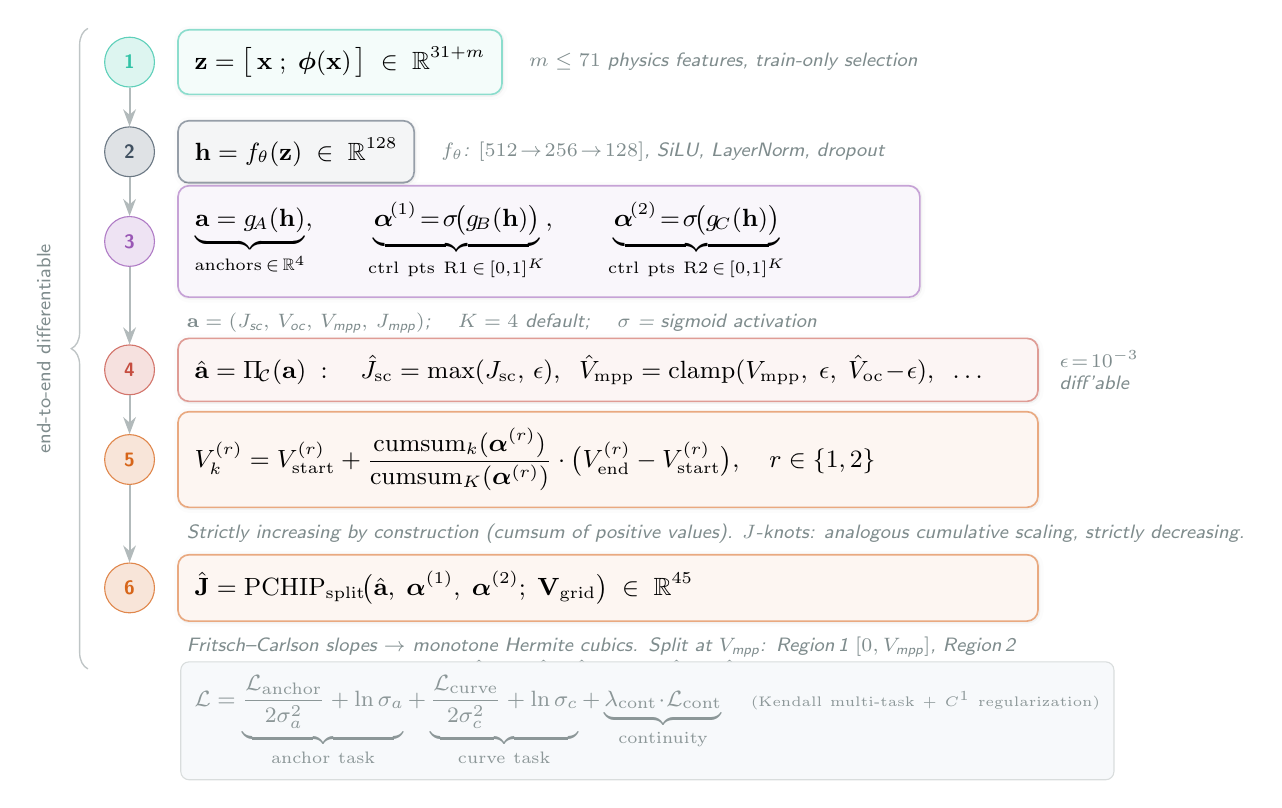
\begin{tikzpicture}[
  >=Stealth,
  every node/.style={font=\small},
  eqbox/.style={
    draw=#1!50,
    fill=#1!5,
    rounded corners=4pt,
    line width=0.6pt,
    inner sep=6pt,
    blur shadow={shadow blur steps=2, shadow xshift=0.3pt, shadow yshift=-0.3pt, shadow opacity=10}
  },
  stepcircle/.style={
    circle, draw=#1!70, fill=#1!15,
    minimum size=18pt, font=\sffamily\scriptsize\bfseries, text=#1!90,
    inner sep=0pt
  },
  steparrow/.style={
    ->, line width=0.7pt, color=annotgray!60
  },
  annot/.style={font=\sffamily\scriptsize\itshape, text=annotgray},
]

% ═══════════════════════════════════════════
% STEP 1: Feature Extraction
% ═══════════════════════════════════════════
\node[stepcircle=featureteal] (s1) at (0, 0) {1};

\node[eqbox=featureteal, right=8pt of s1] (eq1) {
  $\displaystyle \mathbf{z} = \bigl[\,\mathbf{x}\;;\;\boldsymbol{\phi}(\mathbf{x})\,\bigr]
  \;\in\;\mathbb{R}^{31+m}$
};

\node[annot, right=6pt of eq1] {
  $m \le 71$ physics features, train-only selection
};

% ═══════════════════════════════════════════
% STEP 2: Shared Backbone
% ═══════════════════════════════════════════
\node[stepcircle=stepblue, below=14pt of s1] (s2) {};
\node[font=\sffamily\scriptsize\bfseries, text=stepblue!90] at (s2) {2};

\node[eqbox=stepblue, right=8pt of s2] (eq2) {
  $\displaystyle \mathbf{h} = f_\theta(\mathbf{z})
  \;\in\;\mathbb{R}^{128}$
};

\node[annot, right=6pt of eq2] {
  $f_\theta$: $[512 \!\to\! 256 \!\to\! 128]$, SiLU, LayerNorm, dropout
};

% ═══════════════════════════════════════════
% STEP 3: Multi-Head Outputs
% ═══════════════════════════════════════════
\node[stepcircle=headpurple, below=14pt of s2] (s3) {};
\node[font=\sffamily\scriptsize\bfseries, text=headpurple!90] at (s3) {3};

\node[eqbox=headpurple, right=8pt of s3, text width=9cm] (eq3) {
  $\displaystyle
  \underbrace{\mathbf{a} = g_{\!A}(\mathbf{h})}_{\text{anchors}\,\in\,\mathbb{R}^4},
  \qquad
  \underbrace{\boldsymbol{\alpha}^{\!(1)} \!=\! \sigma\!\bigl(g_{\!B}(\mathbf{h})\bigr)}_{\text{ctrl pts R1}\,\in\,[0,1]^K},
  \qquad
  \underbrace{\boldsymbol{\alpha}^{\!(2)} \!=\! \sigma\!\bigl(g_{\!C}(\mathbf{h})\bigr)}_{\text{ctrl pts R2}\,\in\,[0,1]^K}
  $
};

\node[annot, below=2pt of eq3.south west, anchor=north west] {
  $\mathbf{a} = (J_{\text{sc}},\, V_{\text{oc}},\, V_{\text{mpp}},\, J_{\text{mpp}})$;
  \quad $K = 4$ default;
  \quad $\sigma$ = sigmoid activation
};

% ═══════════════════════════════════════════
% STEP 4: Physics Projection
% ═══════════════════════════════════════════
\node[stepcircle=projred, below=28pt of s3] (s4) {};
\node[font=\sffamily\scriptsize\bfseries, text=projred!90] at (s4) {4};

\node[eqbox=projred, right=8pt of s4, text width=10.5cm] (eq4) {
  $\displaystyle
  \hat{\mathbf{a}} = \Pi_{\!\mathcal{C}}(\mathbf{a})
  \;:\quad
  \hat{J}_{\text{sc}} = \max(J_{\text{sc}},\,\epsilon),\;\;
  \hat{V}_{\text{mpp}} = \operatorname{clamp}(V_{\text{mpp}},\;\epsilon,\;\hat{V}_{\text{oc}}\!-\!\epsilon),\;\;
  \ldots
  $
};

\node[annot, right=4pt of eq4.east, anchor=west, text width=1.2cm, align=left] {
  $\epsilon\!=\!10^{-3}$\\
  diff'able
};

% ═══════════════════════════════════════════
% STEP 5: Monotone Knots via Cumsum
% ═══════════════════════════════════════════
\node[stepcircle=splineorg, below=14pt of s4] (s5) {};
\node[font=\sffamily\scriptsize\bfseries, text=splineorg!90] at (s5) {5};

\node[eqbox=splineorg, right=8pt of s5, text width=10.5cm] (eq5) {
  $\displaystyle
  V_k^{(r)} = V_{\text{start}}^{(r)}
  + \frac{\operatorname{cumsum}_k(\boldsymbol{\alpha}^{(r)})}
         {\operatorname{cumsum}_K(\boldsymbol{\alpha}^{(r)})}
  \cdot \bigl(V_{\text{end}}^{(r)} - V_{\text{start}}^{(r)}\bigr),
  \quad r \in \{1,2\}
  $
};

\node[annot, below=2pt of eq5.south west, anchor=north west] {
  Strictly increasing by construction (cumsum of positive values).
  $J$-knots: analogous cumulative scaling, strictly decreasing.
};

% ═══════════════════════════════════════════
% STEP 6: Split PCHIP Reconstruction
% ═══════════════════════════════════════════
\node[stepcircle=splineorg, below=28pt of s5] (s6) {};
\node[font=\sffamily\scriptsize\bfseries, text=splineorg!90] at (s6) {6};

\node[eqbox=splineorg, right=8pt of s6, text width=10.5cm] (eq6) {
  $\displaystyle
  \hat{\mathbf{J}} = \operatorname{PCHIP}_{\text{split}}\!\bigl(
    \hat{\mathbf{a}},\;\boldsymbol{\alpha}^{(1)},\;\boldsymbol{\alpha}^{(2)};\; \mathbf{V}_{\text{grid}}
  \bigr)
  \;\in\;\mathbb{R}^{45}
  $
};

\node[annot, below=2pt of eq6.south west, anchor=north west, text width=11cm] {
  Fritsch--Carlson slopes $\to$ monotone Hermite cubics.
  Split at $V_{\text{mpp}}$: Region\,1 $[0,V_{\text{mpp}}]$, Region\,2 $[V_{\text{mpp}},V_{\text{oc}}]$.
  Endpoint-enforced: $\hat{J}(0)\!=\!\hat{J}_{\text{sc}}$, $\hat{J}(V_{\text{mpp}})\!=\!\hat{J}_{\text{mpp}}$, $\hat{J}(V_{\text{oc}})\!=\!0$.
};

% ═══════════════════════════════════════════
% CONNECTING ARROWS
% ═══════════════════════════════════════════
\draw[steparrow] (s1.south) -- (s2.north);
\draw[steparrow] (s2.south) -- (s3.north);
\draw[steparrow] (s3.south) -- ++(0,-0.35) -- (s4.north);
\draw[steparrow] (s4.south) -- (s5.north);
\draw[steparrow] (s5.south) -- ++(0,-0.35) -- (s6.north);

% ═══════════════════════════════════════════
% OVERALL BRACE + LABEL
% ═══════════════════════════════════════════
\coordinate (topleft) at ($(s1.north west)+(-0.3, 0.2)$);
\coordinate (botleft) at ($(s6.south west)+(-0.3, -0.8)$);

\draw[
  decorate, decoration={brace, amplitude=6pt, raise=0pt, mirror},
  line width=0.5pt, annotgray!50
] (topleft) -- (botleft)
  node[midway, left=10pt, font=\sffamily\scriptsize, text=annotgray, rotate=90, anchor=south] {
    end-to-end differentiable
  };

% ═══════════════════════════════════════════
% LOSS ANNOTATION (compact, at bottom)
% ═══════════════════════════════════════════
\node[
  draw=annotgray!30, fill=accentbg, rounded corners=3pt,
  font=\footnotesize, text=annotgray!90,
  text width=11.5cm, align=center,
  inner sep=5pt,
  below=0.5cm of eq6.south, anchor=north,
  xshift=0.5cm
] (lossline) {
  $\displaystyle
  \mathcal{L} =
  \underbrace{\frac{\mathcal{L}_{\text{anchor}}}{2\sigma_a^2} + \ln\sigma_a}_{\text{anchor task}}
  +
  \underbrace{\frac{\mathcal{L}_{\text{curve}}}{2\sigma_c^2} + \ln\sigma_c}_{\text{curve task}}
  +
  \underbrace{\lambda_{\text{cont}} \!\cdot\! \mathcal{L}_{\text{cont}}}_{\text{continuity}}
  $
  \hfill {\tiny (Kendall multi-task + $C^1$ regularization)}
};

\end{tikzpicture}
\end{document}
